% kvdlra --- arXiv v1 preprint.
% \documentclass{article} so it compiles WITHOUT the NeurIPS style file (the
% Week-4 header comment; swap in \usepackage{neurips_20xx}[preprint] later).
%
% This is the arXiv v1 story AFTER the September GPU program: the fair 2-bit
% (KIVI-scheme) baseline and the official NVIDIA RULER anchor are now IN the
% paper (Secs. quantbaseline, realistic), and claims are scoped to what they
% left. Purpose: timestamp the online DLRA KV-tracking mechanism against
% contemporaneous 2026 work (MomentKV, ResKV, OjaKV).
%
% Honesty invariants enforced throughout (Week-18/19 review panels):
%  * memory = float-equivalent STORED STATE; stored/persisted state is
%    distinguished from resident memory everywhere (reconstruct-then-attend;
%    workspace ~0.98x, decode residency ~1.06x). Honest fp32-at-rest bytes
%    (0.15x flagship / 0.28x marquee) lead every headline; fp16-equiv secondary.
%  * "beats" ONLY for the Wilson-separated marquee vt vs think-c0.5; "leads"
%    everywhere else; comparators think-c0.5 / palu-r0.5 always named.
%  * the 16K cross-model table is a NON-INFERIORITY result ("no detected loss").
%  * var-track on 1024-dim models is an OPEN LIMITATION, not a solved axis.
%  * min_sv_frac = a relative variant of the CKL truncation tolerance theta,
%    not a new invention; the headline is the rank-siphoning diagnosis.
%  * the online axis was OPENED by OjaKV; BUG occupies it with a near-oracle
%    rank-adaptive integrator + a content-selected exact tier.
%  * stored ratio -> 2r/n (0.125x), NOT zero; the 1/T term is the O(rn+hn)
%    overhead amortizing. "below the 2-bit floor" only for the composed q4 cell.
\documentclass[11pt]{article}
\usepackage[margin=1in]{geometry}
\usepackage{amsmath,amssymb}
\usepackage{booktabs}
\usepackage{graphicx}
\setlength{\emergencystretch}{2em}
\usepackage{placeins}
\usepackage{enumitem}
\usepackage{xcolor}
\usepackage[numbers,sort&compress]{natbib}
\usepackage{hyperref}
\usepackage{url}

\hypersetup{colorlinks=true, linkcolor=blue!45!black, citecolor=blue!45!black,
  urlcolor=blue!45!black}

% \todo{...} renders inline in red; grep '\\todo' to enumerate open items.
\newcommand{\todo}[1]{\textcolor{red}{[\textbf{TODO:} #1]}}

\title{Dynamical Low-Rank Approximation as an Online\\ KV-Cache Compressor}
\author{Hari Krishnan Girikumar\\ \texttt{github.com/kvdlra}}
\date{\today}

\begin{document}
\maketitle

\begin{abstract}
The key/value (KV) cache dominates memory in long-context LLM inference, and the
compression literature is organized around three axes: \emph{evict} tokens,
\emph{quantize} elements, or project onto a \emph{low-rank} subspace. Most
low-rank methods fix the subspace at calibration or in a one-shot prefill pass;
the online, per-sequence axis was opened by OjaKV~\citep{zhu2025ojakv} with
Oja's rule. We track it instead with a numerical-analysis tool built for this
problem: the basis-update \& Galerkin (BUG) integrator for dynamical
low-rank approximation (DLRA), a rank-adaptive online subspace tracker whose
error bound is independent of the smallest tracked singular value. On the
(pre-RoPE) KV stream it is a \emph{near-oracle} streaming approximator---within
$1.01$--$1.03\times$ of the truncated-SVD optimum on real KV, where Oja's rule is
$1.3$--$3\times$ worse. We pair the low-rank ``gist'' (which
carries fluency) with a small \emph{surprise-selected} exact tier (which carries
retrieval), and a warm-up seed that repairs early-context recall. On
Llama-3.1-8B, Qwen2.5-7B and Mistral-7B-v0.3, a single configuration reaches
perfect single- and multi-value 16K retrieval with \emph{no detected loss}
($12/12$ trials, Wilson 95\% acc.\ $\ge 0.758$) at \textbf{$0.15\times$} (Llama/Mistral) to \textbf{$0.28\times$} (Qwen) the
full KV as honest fp32-at-rest \emph{stored state} ($0.085$--$0.149\times$
float-equivalent)---$1.8$--$5\times$ less than the channel-pruning baseline
\texttt{think-c0.5} ($0.75\times$) and the low-rank baseline \texttt{palu-r0.5}
($0.50\times$) at honest bytes ($3.4$--$10\times$ float-equivalent), and
$3.6$--$6.7\times$ less than full KV. On the hardest task, variable tracking at 32K on Llama, our config
\emph{beats} \texttt{think-c0.5} (paired McNemar $p=2.0\times10^{-3}$, $0.94$ vs
$0.31$, $n{=}16$; also Wilson-separated) with a suggestive separation from
\texttt{palu-r0.5} ($0.56$; McNemar $p=0.03$, intervals overlap) at
$1.8$--$2.6\times$ less honest stored state ($0.284\times$)---bytes at which
4-bit KIVI also scores $1.00$ variable-tracking, so the separation is from
ThinK/Palu, not from quantization. We give a mechanistic
account of \emph{where} the method is limited: a rank/context retrieval wall at
$r/n\approx0.25$; a rank-siphoning interaction between surprise selection and the
low-rank tracker (which we diagnose and stabilize with a relative
singular-value floor); and an unresolved weakness on variable-tracking chains for
wide-KV ($n{=}1024$) models. Against a KIVI-scheme 2-bit baseline at matched stored bytes on Llama/Mistral
($0.15$ vs $0.16\times$; on Qwen the flagship costs $0.275\times$, $1.7\times$ the
2-bit arm's bytes), the same config wins multi-value retrieval (pooled over the
three families the paired records favor the flagship $21$ vs $0$; per family
McNemar $p=0.008$--$0.031$) and, at 32K, multi-key on Mistral and
variable-tracking on Qwen, ties single-needle everywhere, and trails or ties on
fluency (on Qwen at 32K its $r{=}64$ gist diverges, perplexity $35.1$ vs $8.2$);
4-bit quantization at twice the bytes is not separated from the flagship in any
cell (it trails only on Mistral variable-tracking on point estimate, $0.25$ vs
$0.50$, at half the bytes) and on Qwen, where the flagship's bytes also reach
4-bit, dominates outright; on the official NVIDIA RULER suite (Llama, 16K) the
flagship and the 2-bit arm are not separated on any task (the flagship trails
$0.79$ vs $0.87$ on average) while eviction at $0.1\times$ collapses. Low-rank compresses a feature axis and
quantization a bit axis, so the two compose: the seeded gist with 4-bit
coordinates reaches $0.048\times$ at 16K and $0.034\times$ at 32K, below any
fixed-bit scalar-quantizer floor, with full single/multi-key retrieval and
$0.83$--$1.00$ multi-value on Llama and Mistral, at a fluency cost (Llama
perplexity roughly doubles, $9.25$/$17.1$ vs $5.31$/$8.33$; variable-tracking
$\le0.83$) and with Qwen diverging. We are explicit that today's storage ratio is not deployed VRAM:
BUG reconstructs then attends, so its decode residency is $\approx1.06\times$
full KV until a fused factored-attention kernel (future work) realizes the
storage win as memory; the measured systems payoff is an $\approx7\times$ smaller persisted cache
($9$--$10\times$ faster warm reload on our pod, $0.13$\,s vs $1.2$\,s at 16K), a
win it shares with quantization; what it does not share is the $1/T$ term---the
$O(rn{+}hn)$ overhead amortizes, so the stored ratio falls from $0.151\times$
(16K) toward its $2r/n=0.125\times$ asymptote ($19\%$ under the 2-bit arm's
$0.156\times$; $0.133\times$ already at 64K), where the flagship still retrieves all four tasks
($n{=}8$; no contrast separates) while the quantizer's ratio is nearly flat.
\end{abstract}

\section{Introduction}
\label{sec:intro}

The KV cache of an autoregressive transformer grows linearly with context and,
past a few thousand tokens, exceeds the model weights themselves in memory. The
compression literature falls into three families. \textbf{Eviction} keeps a
budgeted subset of tokens and discards the rest, ranked by attention mass or a
proxy for it (H2O~\citep{zhang2023h2o}, Scissorhands~\citep{liu2023scissorhands},
SnapKV~\citep{li2024snapkv}, PyramidKV~\citep{cai2024pyramidkv},
Quest~\citep{tang2024quest}, Expected Attention~\citep{devoto2025expected}).
\textbf{Quantization} keeps every token but at fewer bits per element
(KIVI~\citep{liu2024kivi}, KVQuant~\citep{hooper2024kvquant},
CacheGen~\citep{liu2024cachegen}). \textbf{Low-rank} methods keep every token but
project the KV features onto a shared subspace
(Palu~\citep{chang2025palu}, Eigen~Attention~\citep{saxena2024eigen},
xKV~\citep{chang2025xkv}, MatryoshkaKV~\citep{lin2025matryoshkakv},
LoRC~\citep{zhang2024lorc}; ThinK~\citep{xu2024think} prunes the channel axis, a
closely related structured-low-rank move).

The low-rank family shares one design choice: \emph{the subspace is not updated
as the sequence streams}. Palu, Eigen~Attention, LoRC and MatryoshkaKV learn or
calibrate a projection offline; xKV extracts shared singular vectors in a
one-shot pass over the prefilled KV (per-sequence, but static thereafter). None
tracks the subspace \emph{online, incrementally}, as tokens arrive. Yet the KV
stream of a single long document is a
\emph{non-stationary} low-rank matrix---its dominant directions drift as topic
and structure change---which is precisely the object dynamical low-rank
approximation (DLRA) was invented to track. DLRA evolves a low-rank
factorization $U S V^\top$ under a matrix flow; the Ceruti--Lubich
basis-update~\& Galerkin (BUG) integrator~\citep{ceruti2022unconventional} and
its rank-adaptive extension~\citep{ceruti2022rankadaptive} do so with an error
bound that is \emph{independent of the smallest tracked singular value}, the
property that makes naive $(U,S,V)$ ODE schemes stiff. That robustness is what a
streaming KV compressor needs when the spectrum is heavy-tailed and the tail
directions are near-null.

\paragraph{This paper.} We turn the BUG integrator into an \emph{online,
training-free, per-sequence} KV compressor and characterize it honestly.

\begin{itemize}[leftmargin=1.4em]
\item A streaming rank-adaptive BUG subspace tracker for the column-streamed KV
matrix, operating pre-RoPE, which is a \emph{near-oracle} low-rank approximator
on real KV (\S\ref{sec:method}, \S\ref{sec:oracle}).
\item A cache built on it: the low-rank ``gist'' plus a \emph{surprise-selected}
exact tier for the sharp facts a summary reproduces worst, plus attention sinks,
a recent ring, and a warm-up seed for early-context recall (\S\ref{sec:cache}).
\item A cross-model result: one configuration reaches perfect single/multi-value
16K retrieval with \emph{no detected loss} on three model families at
$0.085$--$0.149\times$ stored state, and, at 32K on the hardest task, \emph{beats}
the channel-pruning baseline \texttt{think-c0.5} (Wilson-separated) and
\emph{leads} the low-rank baseline \texttt{palu-r0.5} (suggestive under the paired
test) at $1.8$--$2.6\times$ less honest stored state (\S\ref{sec:xmodel}, \S\ref{sec:marquee}).
\item A mechanistic map of the limits: the $r/n\approx0.25$ retrieval wall, the
rank-siphoning tier--gist interaction (diagnosed, and stabilized by a relative
singular-value floor that is a variant of the published CKL truncation
tolerance), and the wide-KV variable-tracking weakness (\S\ref{sec:siphon},
\S\ref{sec:limits}).
\item An honest memory account that separates \emph{stored state} from
\emph{resident memory} and reports both a fp16-equivalent and a fp32-at-rest
ratio, plus a measured persisted-cache cold start (\S\ref{sec:memory}).
\item The crux comparison: a KIVI-scheme 2-bit baseline at matched stored
bytes, paired needle-for-needle, which bounds the contribution honestly---BUG
buys multi-value (and at 32K multi-key on Mistral, variable-tracking on Qwen)
retrieval that 2-bit quantization loses; 4-bit quantization at twice the bytes is
not separated from it in any cell; and the composed
gist-plus-4-bit-coordinates cell reaches $0.048\times$, below any fixed-bit
scalar-quantizer floor, at a fluency cost
(\S\ref{sec:quantbaseline}, \S\ref{sec:subcliff}).
\end{itemize}

\paragraph{Scope and concurrency.} This is an arXiv v1 timestamp of the
mechanism. Two 2026 works---MomentKV~\citep{momentkv2026}, which corrects a
directional gap left by eviction, and ResKV~\citep{reskv2026}, which reconstructs
omitted attention from a residual cache---are independent contemporaneous work;
both augment eviction with lightweight statistics rather than tracking an adaptive
subspace. The online per-sequence low-rank axis itself is not empty---OjaKV
\citep{zhu2025ojakv} tracks it with Oja's rule---but the DLRA integrator
(near-oracle where Oja is $1.3$--$3\times$ worse), the content-selected exact tier
and the mechanistic map are ours. This version adds the two baselines the first
draft lacked---a
KIVI-scheme 2-bit quantizer at matched bytes (\S\ref{sec:quantbaseline}) and an
official NVIDIA RULER anchor (\S\ref{sec:realistic})---and reports what they
took away as plainly as what they left. What it still does \emph{not} contain
is a fused low-rank attention kernel; \S\ref{sec:limits} scopes that.

\section{Method}
\label{sec:method}

\paragraph{Convention.} A per-layer key tensor of shape $(H, T, D)$ is treated
as a matrix $M \in \mathbb{R}^{n \times T}$ with rows $=$ features
($n = H D$; e.g.\ $n{=}1024$ for Llama-3.1-8B and Mistral-7B, $n{=}512$ for
Qwen2.5-7B under GQA) and columns $=$ tokens. A new token is a new column;
values are handled identically.

\subsection{Streaming BUG subspace tracker}
\label{sec:tracker}
We maintain an orthonormal basis $U \in \mathbb{R}^{n \times r}$ and a
square-root core $B$ with $B B^\top = U^\top M M^\top U$. Each new block $C$ of
$b$ columns triggers one augmented rank-adaptive BUG step
\citep{ceruti2022rankadaptive}: (i) compute coordinates $A = U^\top C$ and the
out-of-basis residual $R_\perp = C - U A$; (ii) \emph{range-augment} by a QR of
$R_\perp$, $U_{\text{aug}} = [\,U \mid Q\,]$; (iii) form the grown square-root
core $B_{\text{aug}} = \left[\begin{smallmatrix} B & A \\ 0 & R
\end{smallmatrix}\right]$; (iv) \emph{truncate} via an SVD of $B_{\text{aug}}$,
keeping the leading directions up to a rank cap $r$ and/or a Frobenius-tail
tolerance $\theta$. The reconstruction is the orthogonal projection $\hat M = U
U^\top M$. The block size interpolates between exact and cheap: $b{=}1$ is the
per-token tracker, $b{=}T$ is a single step $=$ the truncated-SVD oracle; on real
KV all block sizes agree to $1$--$3\%$, so we use large blocks for GPU
throughput. To keep admitted directions orthogonal at machine precision when the
residual is numerically tiny (an incoming block already inside the tracked
subspace), we re-orthogonalize $R_\perp$ once against $U$ and rank-reveal it by
SVD, admitting only directions above $100\,\varepsilon\,\|C\|_F$. All core linear
algebra runs in fp32 even when storage is bf16 (bf16 \emph{core} math is
unsafe).

\paragraph{Relation to incremental SVD and sketching.} For a rank-one column
increment the augmented BUG step reduces to the classical incremental-SVD
update---append the incoming column's coordinates to the core, re-factor the
small augmented matrix, keep the leading directions~\citep{brand2006fast}---and
the blocked truncation is a deterministic sketch in the spirit of Frequent
Directions~\citep{liberty2013simple}. What the DLRA framing adds is the
\emph{rank-adaptive} truncation criterion (the Frobenius-tail tolerance $\theta$
of \citet{ceruti2022rankadaptive} and our relative floor, \S\ref{sec:floor}) and
the $\sigma_{\min}$-independent error bound; the near-oracle quality we report
(\S\ref{sec:oracle}) is a \emph{measurement} on real KV, not a theorem for this
column-stream setting. Online basis tracking by Oja's
rule~\citep{oja1982simplified} is the classical alternative (and the OjaKV
baseline~\citep{zhu2025ojakv}); the BUG tracker is near-oracle where it is
$1.3$--$3\times$ worse (\S\ref{sec:oracle}).

\subsection{Pre-RoPE operating point}
\label{sec:prerope}
HuggingFace caches keys \emph{after} rotary position embedding (RoPE), which are
markedly less low-rank than the pre-RoPE keys. We factor the recomputed pre-RoPE
keys and re-apply RoPE to the reconstruction, roughly halving the reconstruction
error at matched rank. (Pre-RoPE key handling is independently exploited by
KVQuant~\citep{hooper2024kvquant} for quantization outliers and by
ShadowKV~\citep{sun2024shadowkv}, which caches a per-sequence low-rank
factorization of the pre-RoPE keys; here it improves rank efficiency.)

\subsection{The cache: gist $+$ surprise-selected exact tier $+$ seed}
\label{sec:cache}
The tracker alone reproduces bulk text but blurs the sharp, low-frequency facts a
retrieval task probes---a planted needle stops being representable once the gist
is a smooth summary of the whole history. We therefore store, per layer, four
bounded parts, all charged in one float-equivalent unit:
\begin{enumerate}[leftmargin=1.6em]
\item the first $n_{\text{sink}}$ tokens verbatim (attention
sinks~\citep{xiao2024streamingllm});
\item a recent ring of the last $W$ tokens verbatim (local context is exact);
\item the \emph{gist}: the tracked $(U, B)$ plus up to a budgeted set of
per-token coordinate columns $C = U^\top M$ ($r$ floats/token instead of $n$);
\item an \emph{exact tier} of up to $h$ tokens kept verbatim, selected by
\emph{surprise}---the out-of-subspace residual $\|k - U U^\top k\|/\|k\|$, i.e.\
exactly the tokens the low-rank gist reproduces worst.
\end{enumerate}
Perplexity rides mostly on the gist; needle retrieval rides mostly on the exact
tier. The two fail independently, which is the lever the rest of the paper pulls.
Because softmax attention needs per-token information for every attendable token,
a \emph{bounded}-memory variant bounds the attended set: when the coordinate
buffer is full, columns are evicted (by attention mass, coordinate energy, or
surprise), and at matched memory the gist retains an $\approx n/r\times$ longer,
approximately represented history than whole-token eviction. The configurations
evaluated here keep the full coordinate buffer (stored state is $\Theta(T)$ with a
$2r/n$ slope, \S\ref{sec:memory}); coordinate eviction is not exercised at these
contexts.

\paragraph{Warm-up seed.} The first ingest chunk originally bypassed the exact
tier, so the earliest-planted facts were structurally lost---the ``warm-up
window'' that made the family a $\ge$32K-only method. Routing the first chunk
through the same surprise path (scored against the strictly-older, needle-free
basis) repairs 16K recall (\S\ref{sec:xmodel}); it is default-off and evaluated
as an ablation.

\paragraph{Score-rank decoupling.} At high gist rank the surprise score itself
degrades: a large $U$ ``fits'' a planted needle into invisibility so it never
enters the exact tier. Capping the \emph{selection} scoring to a leading
rank-$s$ subview of $U$ (default-off, zero extra memory, $+0.3\%$ perplexity)
un-blinds selection without shrinking the gist. This knob (denoted \texttt{-s}$s$)
recovers Llama's $r{=}128$ retrieval and underlies the marquee config
(\S\ref{sec:marquee}); it does \emph{not} rescue Qwen (\S\ref{sec:siphon}).

\subsection{Stability: a relative singular-value floor (a CKL-$\theta$ variant)}
\label{sec:floor}
With no truncation tolerance, the rank-adaptive step always pads the basis to the
rank cap, and on an ill-conditioned KV stream those near-null tail directions can
tip into a numerical explosion. The rank-adaptive integrator already provides the
principled remedy---the Frobenius-tail tolerance $\theta$ of
\citet{ceruti2022rankadaptive}, which drops directions whose discarded singular
tail falls below an \emph{absolute} threshold. We use a \emph{relative},
self-scaling variant, \texttt{min\_sv\_frac}: after truncation, additionally drop
directions whose singular value is $\le$ a fraction of the leading one, capping
the tracked rank at the block's numerical rank with no per-stream tuning. This is
a small variant of published DLRA truncation, not a new mechanism; it is
default-off and bit-for-bit identical when off. Its value is diagnostic and
practical (\S\ref{sec:siphon}): it removes a whole class of high-rank divergence
and thereby extends the numerically usable rank on non-Llama families.

\subsection{Composition with quantization}
\label{sec:quant}
Low-rank compresses the \emph{feature} axis; quantization compresses the
\emph{bit} axis. They are orthogonal and multiply: the gist stores $U$
($n\times r$) and coordinates $C$ ($r \times T$), and $C$'s columns can be
scalar/vector quantized (we use TurboQuant's rotated scalar
quantizer~\citep{zandieh2025turboquant}; low-rank$\times$quantization composition
for KV is also explored by GEAR~\citep{kang2024gear} and Palu). Because BUG
factors are pre-RoPE, the quantization rotation and RoPE never need to commute
(RoPE is applied last). We report the composition on 1B in \S\ref{sec:frontier}
and, on 7B/8B, a head-to-head against a dedicated 2-bit KV quantizer
(\S\ref{sec:quantbaseline}); the axes compose (\S\ref{sec:subcliff}) rather than
low-rank dominating quantization.

\section{Related work}
\label{sec:related}

\paragraph{Eviction.} H2O~\citep{zhang2023h2o},
Scissorhands~\citep{liu2023scissorhands} and SnapKV~\citep{li2024snapkv} rank
tokens by (proxies for) attention mass; PyramidKV~\citep{cai2024pyramidkv} varies
the budget by layer; Quest~\citep{tang2024quest} selects KV pages per query;
Expected~Attention~\citep{devoto2025expected} scores tokens by the attention
future queries are expected to pay. Eviction is near-lossless at moderate budgets
and, unlike us, genuinely shrinks resident memory. Its weakness is the extreme
band: it degrades on tasks needing many linked tokens and, at $\le0.1\times$,
loses the hardest retrieval (\S\ref{sec:xmodel}). \emph{Naming note:} ``EA''
is overloaded---Expected~Attention~\citep{devoto2025expected} (an eviction score,
and the eviction baseline in our tables) is distinct from Eigen~Attention
\citep{saxena2024eigen} (a low-rank projection). We write the names in full.

\paragraph{Quantization.} KIVI~\citep{liu2024kivi} (per-channel keys, per-token
values, 2-bit) and KVQuant~\citep{hooper2024kvquant} (pre-RoPE, non-uniform,
dense-and-sparse) reach $\approx0.125$--$0.19\times$ near-losslessly;
CacheGen~\citep{liu2024cachegen} targets the network/serving path. This family
most directly contests our headline band, so we run a paired KIVI-scheme 2-bit
(and 4-bit) baseline against it (\S\ref{sec:quantbaseline}) and compose with it
below the 2-bit floor (\S\ref{sec:subcliff}).

\paragraph{Low-rank / factorization.} Palu~\citep{chang2025palu} decomposes the
KV projections and caches low-rank latents; Eigen~Attention~\citep{saxena2024eigen}
runs attention in a fixed low-rank space; xKV~\citep{chang2025xkv} shares
singular vectors across layers; MatryoshkaKV~\citep{lin2025matryoshkakv} trains
nested orthogonal projections; LoRC~\citep{zhang2024lorc} does progressive
weight-matrix low-rank; ThinK~\citep{xu2024think} prunes key channels;
ShadowKV~\citep{sun2024shadowkv} caches a per-sequence one-shot low-rank
factorization of the pre-RoPE keys with offloaded values.
Multi-head latent attention (MLA) in DeepSeek-V2~\citep{deepseekv2} bakes a
low-rank latent KV into the architecture (train-time). \textbf{Each of these
fixes its subspace statically}---offline, at train time, or in a one-shot prefill
pass (xKV, ShadowKV). The exception is OjaKV~\citep{zhu2025ojakv}, which updates a
per-sequence subspace online with Oja's rule; we differ from it in the tracker (a
near-oracle rank-adaptive DLRA integrator vs.\ Oja's rule, $1.3$--$3\times$ better
at matched memory, \S\ref{sec:oracle}) and in selecting the exact tier by
\emph{content} (surprise) rather than by position.

\paragraph{Closest priors, and how we differ.} Two works combine low-rank with an
exact/sparse component, as we do. LESS~\citep{dong2024less} adds a small
constant-size \emph{learned} low-rank state (tiny per-layer MLPs) to an eviction
policy so evicted tokens remain queryable. LoLA~\citep{mcdermott2025lola}
augments \emph{linear} attention with a sparse global cache for hard-to-memorize
pairs. Both are structurally similar in spirit---a low-rank summary plus an exact
escape hatch---but both use a \emph{fixed or calibration-time} low-rank basis
(LESS learns MLPs; LoLA inherits the linear-attention feature map). We instead
track an \emph{adaptive, per-sequence} subspace online with a DLRA integrator,
and select the exact tier by low-rank \emph{surprise} (the tracker's own
residual) rather than by attention mass---a residual-to-a-tracked-subspace
statistic with a long lineage in adaptive sampling. The surprise coupling is what
makes the exact tier self-consistent with the gist---and, as \S\ref{sec:siphon}
shows, is also the source of the one interaction we had to diagnose.

\paragraph{DLRA lineage.} DLRA originates with Koch \&
Lubich~\citep{koch2007dlra}; the robust integrators we use are
Ceruti--Lubich~\citep{ceruti2022unconventional} and the rank-adaptive
Ceruti--Kusch--Lubich~\citep{ceruti2022rankadaptive}. DLRA has been used to
compress \emph{weights} during training (``low-rank lottery
tickets''~\citep{schotthofer2022lottery};
robust compression~\citep{schotthofer2025robust}); we appear to be the first to
use it as an \emph{inference-time, streaming} compressor of the \emph{activation}
KV cache. Our stability floor (\S\ref{sec:floor}) is a relative variant of the
rank-adaptive tolerance in~\citep{ceruti2022rankadaptive}.

\paragraph{Contemporaneous 2026 work.} MomentKV~\citep{momentkv2026} keeps compact
moment statistics of the evicted set to correct the attention direction;
ResKV~\citep{reskv2026} splits a fixed budget into an exact cache plus a residual
that reconstructs omitted attention mass. Both are eviction-plus-correction; both
keep the retained tokens exact and summarize only the discarded remainder---as do
the cache-merging methods CaM~\citep{zhang2024cam} and
KVMerger~\citep{wang2024kvmerger}. Our gist summarizes the \emph{bulk} in an
adaptive subspace and keeps only the \emph{surprising} tokens exact---the
complementary decomposition. MomentKV's token score is, like our surprise, a
residual norm against a summary subspace; ours is measured against a rank-adaptive
\emph{tracked} basis and the selected tokens are kept exact rather than corrected.
These are independent contemporaneous work, not evaluated baselines.

\section{Experiments}
\label{sec:exp}

\paragraph{Setup.} Models: Llama-3.1-8B-Instruct~\citep{grattafiori2024llama3}
(ungated \texttt{unsloth} mirror, config-identical), Qwen2.5-7B-Instruct
\citep{qwen2025qwen25}, Mistral-7B-Instruct-v0.3~\citep{jiang2023mistral7b}, and
Llama-3.2-1B-Instruct for the composition study. Retrieval is measured on a
RULER-style~\citep{hsieh2024ruler} generator (single-needle, multi-key,
multi-value, variable-tracking) at 16K/32K; perplexity on held-out windows.
Reported \emph{memory} is a float-equivalent \emph{stored-state} ratio unless
stated otherwise (\S\ref{sec:memory} separates this from resident memory). The
baselines \texttt{think-c0.5}~\citep{xu2024think}, \texttt{palu-r0.5}
\citep{chang2025palu} and Expected~Attention~\citep{devoto2025expected} are run
through NVIDIA's kvpress~\citep{nvidia2024kvpress}. We
give Wilson 95\% intervals on retrieval cells and per-window NLL on perplexity;
$12/12$ trials corresponds to a Wilson lower bound of $0.758$. Unless noted,
retrieval cells use $n{=}12$ ($6$ trials $\times\,2$ seeds) and the marquee uses
$n{=}16$ ($8\times2$); some 32K composition cells and the 1B study are lower-$n$
and flagged as such. Per-trial hit records for every headline cell are released
(\texttt{results/w18\_pertrial/} and \texttt{results/w19\_pertrial/}), and the
runs' git-SHA/GPU/library environment is in
\texttt{results/w18-env-provenance.txt} and
\texttt{results/w19-env-provenance.txt}. The generator uses a small fixed
filler pool by default (an external-validity caveat, \S\ref{sec:limits}); a
per-family seed/window/depth appendix table is deferred to the camera-ready.

\subsection{Near-oracle streaming reconstruction}
\label{sec:oracle}
On real Llama-3.2-1B KV, the streaming BUG tracker matches the truncated-SVD
(Eckart--Young~\citep{eckart1936approximation}) optimum to within
$1.01$--$1.03\times$ at every rank, beats fixed-rank incremental
SVD~\citep{brand2006fast} everywhere, and beats Oja's
rule~\citep{oja1982simplified,zhu2025ojakv} by $1.3$--$3.0\times$; the pre-RoPE
operating point roughly halves the error at matched budget. The tracker is thus a faithful online stand-in for the
offline optimum---the property the fixed-subspace baselines obtain only by
calibration.
% source: docs (Week-2), README "near-oracle (within ~1.01-1.03x of truncated SVD)".

\subsection{Cross-model 16K retrieval: no detected loss at $0.085$--$0.149\times$}
\label{sec:xmodel}
Table~\ref{tab:xmodel} reports the single configuration
\texttt{bugSseed-r64-h256} (rank-64 gist, 256-token surprise tier, warm-up seed)
at 16K on three families. On single-needle and multi-value retrieval it scores
$12/12$ on all three---a \textbf{non-inferiority} result: with no observed
failure, the Wilson 95\% interval is $[0.758, 1.0]$, so we can claim
\emph{no detected loss at accuracy $\ge0.76$}, not a match or a win. There are
\emph{zero} Wilson-separated flagship-vs-\texttt{think}/\texttt{palu} cells in
either direction at 16K (the flagship does separate from the 2-bit quantizer on
multi-value, \S\ref{sec:quantbaseline}). What is notable is \emph{where} this holds: at $0.085$--$0.149\times$ stored
state, i.e.\ $3.4$--$10\times$ less than \texttt{think-c0.5} ($0.75\times$) and
\texttt{palu-r0.5} ($0.50\times$), and $6.7$--$13\times$ less than full KV. BUG
does \emph{not} win on perplexity here---its fluency is above the baselines'
(r64 perplexity is $1.08$--$1.32\times$ full)---the edge is stored state at
matched retrieval. On multi-value it \emph{leads} the baselines on point
estimate (Qwen 16K: $1.00$ vs \texttt{think-c0.5} $0.83$ / \texttt{palu-r0.5}
$0.92$), but this is not Wilson-separated and we do not call it a win.
% source: docs/week17-explained.md sec.1 table (n=12), docs/week16-handover.md sec.2 baselines.

\begin{table}[t]
\centering
\caption{Cross-model 16K retrieval, config \texttt{bugSseed-r64-h256}, $n{=}12$
(Wilson 95\%). Single/multi-value are $12/12$ on all three families (no detected
loss). Variable-tracking is an open limitation on the two wide-KV ($n{=}1024$)
models (\S\ref{sec:limits}). Memory is float-equivalent stored state.}
\label{tab:xmodel}
\begin{tabular}{lccccc}
\toprule
model & feat.\ $n$ & single & multi-value & var-track & stored state \\
\midrule
Qwen2.5-7B        & 512  & $1.00\,[0.76,1.0]$ & $1.00\,[0.76,1.0]$ & $\mathbf{1.00}\,[0.76,1.0]$ & $0.149\times$ \\
Mistral-7B-v0.3   & 1024 & $1.00\,[0.76,1.0]$ & $1.00\,[0.76,1.0]$ & $0.50\,[0.25,0.75]$          & $0.085\times$ \\
Llama-3.1-8B      & 1024 & $1.00\,[0.76,1.0]$ & $1.00\,[0.76,1.0]$ & $0.58\,[0.32,0.80]$          & $0.085\times$ \\
\bottomrule
\end{tabular}
\end{table}

\paragraph{32K firming ($n{=}12$).} The same configuration was re-run at 32K on
all three families at full sample size (Table~\ref{tab:xmodel32}), firming what
were previously $n{=}4$ point estimates. Single- and multi-key retrieval hold at
$12/12$ on all three; multi-value holds ($12/12$) on Qwen and Llama and is
$0.83\,[0.55,0.95]$ on Mistral; variable-tracking is $1.00$ on Qwen,
$0.92\,[0.65,0.98]$ on Llama, and $0.42\,[0.19,0.68]$ on Mistral. Two honest
notes travel with the 32K point: Qwen's \emph{fluency} at $r{=}64$ degrades at
32K (perplexity $8.2\to35.1$ from 16K, while retrieval stays $1.00$), so the
natural 32K operating point for Qwen is a higher rank with the stability floor of
\S\ref{sec:floor}; Mistral and Llama perplexity stay healthy ($3.76$, $8.33$).
The var-track ordering is the same wide-KV story as 16K (Qwen $n{=}512$ perfect;
the $n{=}1024$ models weaker), discussed in \S\ref{sec:limits}.
% source: results/w18-g1-report.md (32K n=12: Qwen 1/1/1/1 @0.139x ppl35.08; Llama 1/1/1/0.92 @0.075x ppl8.33; Mistral 1/1/0.83/0.42 @0.075x ppl3.76).

\begin{table}[t]
\centering
\caption{32K retrieval, config \texttt{bugSseed-r64-h256}, $n{=}12$ (Wilson 95\%),
firming the previously $n{=}4$ cells. Memory is float-equivalent stored state.}
\label{tab:xmodel32}
\small
\begin{tabular}{lccccc}
\toprule
model & single & multi-key & multi-value & var-track & stored state \\
\midrule
Qwen2.5-7B      & $1.00\,[0.76,1.0]$ & $1.00\,[0.76,1.0]$ & $1.00\,[0.76,1.0]$ & $\mathbf{1.00}\,[0.76,1.0]$ & $0.139\times$ \\
Mistral-7B-v0.3 & $1.00\,[0.76,1.0]$ & $1.00\,[0.76,1.0]$ & $0.83\,[0.55,0.95]$ & $0.42\,[0.19,0.68]$          & $0.075\times$ \\
Llama-3.1-8B    & $1.00\,[0.76,1.0]$ & $1.00\,[0.76,1.0]$ & $1.00\,[0.76,1.0]$ & $0.92\,[0.65,0.98]$          & $0.075\times$ \\
\bottomrule
\end{tabular}
\end{table}

\subsection{Marquee: variable tracking at 32K on Llama}
\label{sec:marquee}
The one separated retrieval result is the hardest task on the largest model. At
32K on Llama-3.1-8B, \texttt{bugSseed-r128-h1024-s32} (the score-rank config,
$0.284\times$ honest stored state, $0.16\times$ float-equivalent, $n{=}16$) scores
variable-tracking $0.94\,[0.72,0.99]$
and multi-value $1.00\,[0.81,1.0]$. Because all arms are scored on the
\emph{same} needles (shared \texttt{seed$\cdot$131+trial} layout), the correct
contrast is the paired McNemar test, which we compute from the committed
per-trial records. Against the $n{=}16$ baselines
(Table~\ref{tab:marquee}): it \textbf{beats} \texttt{think-c0.5}
($0.31\,[0.14,0.56]$; $10$ discordant pairs, all favoring BUG; McNemar exact
$p=2.0\times10^{-3}$, Wilson intervals also disjoint, $0.72>0.56$) at
$1.8$--$2.6\times$ less honest stored state. It also separates from \texttt{palu-r0.5}
under the same paired test ($0.56\,[0.33,0.77]$; $6$ discordant, all favoring BUG;
$p=3.1\times10^{-2}$), but we report this only as \emph{suggestive}: the Wilson
intervals overlap and, unlike the \texttt{think-c0.5} contrast, it does not
survive a family-wise correction. Multi-value is a three-way tie at $1.00$. At
these honest bytes ($0.284\times$) the marquee is byte-matched with the 4-bit KIVI
arm, which scores variable-tracking $1.00$ ($12/12$) at 32K
(Table~\ref{tab:official}); the marquee's separation is therefore from
ThinK/Palu, not from quantization. The
honest headline is therefore ``\emph{beats the channel-pruning baseline
\texttt{think-c0.5} on the hardest task (paired, multiple-comparison-robust), with
a suggestive separation from the low-rank baseline \texttt{palu-r0.5}, at
several-fold less stored state}.''

\paragraph{Multiple comparisons.} The retrieval tables report $\sim$40 descriptive
Wilson cells; we treat the 32K-Llama variable-tracking contrast as the single
\emph{pre-registered confirmatory} comparison (registered in the pod matrix before
the run), so the \texttt{think-c0.5} $p=2.0\times10^{-3}$ needs no family-wise
inflation. All other cross-arm comparisons, including the \texttt{palu-r0.5}
separation, are exploratory.
% source: results/w18-g4-marquee-contrasts.json (McNemar from w18_pertrial/g4-llama-trials.txt: think 10/0 discordant p=0.0020, palu 6/0 p=0.0312, n=16); pre-registration = scripts/pod/w18.sh MODE=g4.

\begin{table}[t]
\centering
\caption{Marquee (Llama-3.1-8B, 32K variable-tracking, $n{=}16$, Wilson 95\% +
paired McNemar vs.\ flagship). The \texttt{think-c0.5} contrast is the
pre-registered confirmatory comparison (McNemar $p{=}2.0\!\times\!10^{-3}$, also
Wilson-disjoint); \texttt{palu-r0.5} separates under the paired test
($p{=}3.1\!\times\!10^{-2}$) but Wilson intervals overlap, so it is reported as
suggestive; 4-bit KIVI at the same honest bytes matches it. Memory is honest
stored state (fp32-at-rest).}
\label{tab:marquee}
\small
\begin{tabular}{lcccc}
\toprule
config & var-track (Wilson 95\%) & stored state & McNemar $p$ & vs.\ flagship \\
\midrule
\texttt{bugSseed-r128-h1024-s32} & $\mathbf{0.94}\,[0.72,0.99]$ & $0.284\times$ & --- & --- \\
\texttt{think-c0.5}              & $0.31\,[0.14,0.56]$          & $0.75\times$ & $2.0\!\times\!10^{-3}$ & beats (confirmatory) \\
\texttt{palu-r0.5}               & $0.56\,[0.33,0.77]$          & $0.50\times$ & $3.1\!\times\!10^{-2}$ & leads (suggestive) \\
KIVI 4-bit                       & $1.00\,[0.76,1.0]$          & $0.284\times$ & --- & tie (same bytes) \\
\bottomrule
\end{tabular}
\end{table}

Perplexity is a tie with the compression field, not with full KV, and---unlike an
earlier draft---the marquee perplexity and retrieval are now measured on the
\emph{same pod in the same run}, removing the cross-run provenance caveat. At 32K
on Llama over identical windows ($n{=}8$): full $6.975$, \texttt{think-c0.5}
$7.196$, \texttt{palu-r0.5} $7.232$, \texttt{bugSseed-r128-s32} $7.353$---within
the pre-registered $0.05$-bits/token band of both compressors ($+0.031$/$+0.024$
bits/token vs.\ think/palu) but $+0.076$ over uncompressed full KV. At 16K the
arms are within the same band. (Perplexities are quoted to the scorer's
resolution; per-window NLL was summed in bf16 in these runs, a
$\approx0.006$-bit/token floor below which sub-band gaps are not resolved, since
fixed to fp32.) Two baseline numbers here were originally our
own port defects, found and fixed in the baselines' favor before this comparison
(a ShadowKV decode-scope bug; a Palu attention-sink low-ranking that had inflated
its perplexity from $7.232$ to $9.236$); we report the corrected values.
% source: results/w18-g4-llama (SAME-POD n=8 ppl this run: full 6.975, think-c0.5 7.196, palu-r0.5 7.232, bugSseed-r128-s32 7.353 -- confirms the Week-15 values, now same-run; retrieval n=16 same pod: vt 0.94 vs think 0.31 / palu 0.56).

\subsection{The rank-siphoning diagnosis and the $r/n\approx0.25$ wall}
\label{sec:siphon}
Pushing the gist rank up does \emph{not} monotonically help, and the reason is a
mechanism worth naming. \textbf{The $r/n\approx0.25$ retrieval wall.} Retrieval
collapses to zero once the gist rank reaches about a quarter of the feature
dimension: Llama ($n{=}1024$) collapses at $r{=}256$, Qwen ($n{=}512$) at
$r{=}128$---both $r/n = 0.25$. A larger gist is a \emph{smoother} summary, so a
planted needle stops looking surprising, never enters the exact tier, and is lost.
This is a dimensionless onset, supported by a matched control: a seeded
\texttt{bugSseed-r256-h1024} column on Llama ($r/n{=}0.25$) scores
$0.00$ on \emph{all four} 32K tasks at $n{=}12$ (single/multi-key/multi-value/
variable-tracking; this run), exactly like Qwen at $r{=}128$.
% source: results/w18-g4-llama r256 control (32K n=12: all four tasks 0.00 @0.284x).
% source: docs/week11-decision-table.md (r256 = 0), docs/week16-explained.md (r/n wall), review-meta-verdict.

\textbf{Rank siphoning.} Separately, coupling surprise selection to the low-rank
tracker can \emph{starve} the tracker: the exact tier pulls the rank-carrying,
high-surprise tokens \emph{out} of the gist, dropping its effective rank below
the cap, whereupon the rank-adaptive step pads with near-null tail directions
that tip into numerical divergence at high rank. This showed up as several
unexplained blow-ups (Qwen \texttt{bug-r256} perplexity $27{,}531$; the ``puzzle''
where a \emph{larger} exact tier destroyed fluency, Qwen
\texttt{bugSseed-r128-h1024} $=714$; Mistral \texttt{bug-r128} $=138$). The
relative singular-value floor of \S\ref{sec:floor} (\texttt{-{}-min-sv-frac 1e-2})
removes the entire class (Table~\ref{tab:floor}); on Mistral fluency then improves
monotonically with rank ($6.22\to5.57\to5.23$ at $r{=}64/128/256$), so the floor
does not merely rescue divergence---it extends the numerically usable rank. This
is a within-method stability property (a floored high-rank cell is still
Palu-dominated at matched memory), reported as a diagnosis, not a frontier claim.
% source: docs/week17-explained.md sec.3 (floor table), streaming_torch.py min_sv_frac.

\begin{table}[t]
\centering
\caption{The relative singular-value floor (\texttt{-{}-min-sv-frac 1e-2},
default-off) converts high-rank divergence into healthy fluency (16K perplexity).
Default-off and bit-identical when off; retrieval- and footprint-neutral at the
operating point.}
\label{tab:floor}
\begin{tabular}{lcc}
\toprule
16K perplexity & floor off & floor on \\
\midrule
Qwen \texttt{bug-r256}                    & $27{,}531.7$ & $\mathbf{6.995}$ \\
Qwen \texttt{bugSseed-r128-h1024} (puzzle)& $714.4$      & $\mathbf{6.941}$ \\
Mistral \texttt{bug-r128}                 & $138.3$      & $\mathbf{5.574}$ \\
Mistral \texttt{bug-r256}                 & $37.2$       & $\mathbf{5.226}$ \\
Mistral \texttt{bugSseed-r128-h1024}      & $60.4$       & $\mathbf{5.045}$ \\
\bottomrule
\end{tabular}
\end{table}

\subsection{Below the quantizer's floor: the seeded gist with 4-bit coordinates}
\label{sec:subcliff}
A $b$-bit quantizer cannot store fewer than $b/16$ of full KV plus its scale
overhead---$0.156\times$ for the 2-bit arm above. Low-rank has no such floor,
and the two axes compose: keeping $512$ recent gist coordinates in fp32 and
demoting every older coordinate column to 4-bit rotated-scalar (TurboQuant~\S2)
codes (never
dropping it) gives \texttt{bugSseed-r64-h256-q4} at \textbf{$0.048\times$}
stored state (fp32 at rest; $0.042\times$ fp16-equivalent), $3.4\times$ below
the 2-bit arm.\footnote{An earlier Week-18 arm also labeled \texttt{q4} never
quantized---a budget inversion demoted no coordinates, so its rows billed
identically to the unseeded flagship; those rows are annotated invalid
(\texttt{results/w18-g1-report.md}) and are not the cell reported here, which is
the corrected Week-19 \texttt{a1q} run.} At 16K ($n{=}12$, same needles) this cell scores
single/multi-key/multi-value/variable-tracking $= 1.00/1.00/1.00/0.50$ on Llama
and $1.00/1.00/0.92/0.33$ on Mistral---multi-key and multi-value retrieval that
the 2-bit arm at three times the bytes loses ($0.67/0.42$ and $0.58/0.50$).
This is a compression depth no fixed-bit scalar quantizer can be configured to
reach ($0.156\times$ at 2 bits), with retrieval intact on the sharp-needle tasks;
whether an eviction$\times$quantization composite reaches it is not measured here.
At 32K the cell falls to
$0.034\times$ (its $1/T$ term) and holds: Llama $1.00/1.00/1.00/0.83$, Mistral
$1.00/1.00/0.83/0.58$---at a fifth of the 2-bit arm's bytes, where that arm
scores $1.00/0.83/0.92/0.92$ (Llama) and $0.83/0.25/0.08/0.00$ (Mistral). Three
qualifications travel with it. It is \emph{family-dependent}: on Qwen the same
arm retrieves nothing ($0/0/0/0$ at $0.071\times$) and its perplexity diverges,
the heavy-tailed Qwen key coordinates defeating 4-bit rotated-scalar codes exactly as
Qwen's key-bias channel defeats per-token key quantization. It \emph{costs
fluency}, more on Llama than on Mistral: Llama perplexity is $9.25$ (16K) and
$17.1$ (32K) against $5.31$/$8.33$ unquantized, Mistral $6.56$/$4.28$ against
$5.50$/$3.76$, so the cell is a retrieval-tier operating point, not a
fluency-preserving one. And variable tracking is no better than at $r{=}64$
unquantized. Channel-pruning (ThinK) and low-rank factorization (Palu), at the
operating points compared (\texttt{think-c0.5}, \texttt{palu-r0.5}), sit at
$0.50$--$0.75\times$; eviction reaches $0.1\times$
(Expected~Attention at $0.100\times$) but its retrieval there is
\emph{family-dependent and unreliable}. In our $n{=}12$ three-family grid at
$0.100\times$ (Table~\ref{tab:evict}), Expected~Attention holds
single/multi-key/multi-value only on Llama---and loses variable-tracking there
($0.08$ at 16K, $0.58$ at 32K)---while on Qwen and Mistral it collapses on most
tasks (single $\le0.50$, multi-key and multi-value $\to0$); \emph{no family
retains all four tasks} at $0.1\times$. SnapKV at $0.100\times$ is weaker still
(multi-key $0.17$--$0.42$, variable-tracking $0$).
% source: results/w19-a1q-{llama,mistral,qwen}-lines.txt (Week-19 a1q pods @1cbc31f: bugSseed-r64-h256-q4 16K+32K n=12; ppl Llama 9.254/17.074, Mistral 6.558/4.280); the Week-18 "q4" rows are NOT this arm (its quant tier never filled; results/w18-g1-report.md annotation). Eviction grid: results/w18-g3-{qwen,mistral,llama}-lines.txt.

\begin{table}[t]
\centering
\caption{Eviction at $0.100\times$ stored state, Expected~Attention
(\texttt{ea-k0.1}), $n{=}12$ (accuracy). Family-dependent and never all-four:
strong on Llama single/multi-key/multi-value, collapsing on Qwen/Mistral, and
losing variable-tracking on every family. Cyclic-filler generator
(\S\ref{sec:realistic} shows it collapses further on realistic text).}
\label{tab:evict}
\begin{tabular}{llcccc}
\toprule
model & ctx & single & multi-key & multi-value & var-track \\
\midrule
Llama-3.1-8B    & 16K & $1.00$ & $0.92$ & $1.00$ & $0.08$ \\
Llama-3.1-8B    & 32K & $1.00$ & $0.92$ & $0.92$ & $0.58$ \\
Qwen2.5-7B      & 16K & $0.17$ & $0.00$ & $0.00$ & $0.00$ \\
Mistral-7B-v0.3 & 16K & $0.50$ & $0.08$ & $0.00$ & $0.00$ \\
\bottomrule
\end{tabular}
\end{table}

\subsection{A fair 2-bit baseline at matched stored bytes}
\label{sec:quantbaseline}
The family that most directly contests the headline band is 2-bit KV
quantization. We ran a KIVI-scheme baseline through the identical harness on
all three families at 16K and 32K ($n{=}12$, the \emph{same} needles as the
flagship so every contrast is paired): keys quantized \emph{per channel} (groups
of 64 tokens per head-dim channel, the scheme that isolates outlier channels),
values \emph{per token}, a 128-token fp16 residual, and scale/zero billed at their
stored 16-bit width---asymptotically $0.156\times$ at 2 bits and $0.281\times$ at
4 bits. This is the HuggingFace/quanto grouping ($G{=}64$); KIVI's paper default
is the finer $G{=}32$ (more accurate, $\approx0.19\times$ at 2 bits), so at matched
bytes ours is a slightly coarser but cheaper 2-bit arm. Prefill for the quant (and
flagship) arms is chunked (4096-token blocks, residual flushed), so this is a KIVI
\emph{scheme} under a streaming protocol rather than KIVI's full-precision-prefill
operating point; the scorer presses and full-KV run use single-shot prefill. An
8-bit control on a second backend (hqq) scores $1.00$ on all four tasks on Llama
and Qwen ($n{=}4$; quanto and hqq agree at 2 bits on Qwen single-needle), so the
decode path is sound. (An earlier draft
reported an off-the-shelf quantized cache at $0.00$ retrieval; that
implementation quantized \emph{keys} per token, which a single large key channel
defeats---on Qwen2.5 one channel carries the key bias---and the zero reproduces
under that scheme while vanishing under the faithful one. The finding is a
configuration hazard of the library default, not a property of quantization.)

\textbf{Retrieval at matched bytes} (Table~\ref{tab:fairquant},
Figure~\ref{fig:fairquant}). On Llama and
Mistral the flagship's honest stored state ($0.151\times$ at 16K, $0.139\times$
at 32K, fp32 at rest) sits next to the 2-bit arm ($0.163\times$/$0.160\times$).
Single-needle retrieval is a tie everywhere. On \emph{multi-value} the flagship
wins on all three families at 16K (paired McNemar: Llama $7$ discordant pairs all
favoring BUG, $p{=}0.016$; Mistral $6/0$, $p{=}0.031$; Qwen $8/0$, $p{=}0.008$),
and at 32K on Mistral (multi-key $9/0$ and multi-value $9/0$, both
$p{=}0.004$) and Qwen (multi-value $10/0$, $p{=}0.002$; variable-tracking $9/0$,
$p{=}0.004$). On Llama at 32K the 2-bit arm is strong ($1.00/0.83/0.92/0.92$)
and no contrast separates (at $n{=}12$ a single-task contrast needs $\ge6$ one-way
discordant pairs to reach $p<0.05$, so these nulls bound rather than establish
equivalence). Variable tracking is mixed: the 2-bit arm leads the
flagship on Llama at 16K ($0.67$ vs $0.58$, $3$ vs $4$ discordant, not
separated) and trails it on Mistral and Qwen.
\textbf{The 4-bit arm} ($0.287\times$/$0.284\times$) is not separated from the
flagship in any cell (it leads on Llama 16K variable-tracking, $5/0$, $p{=}0.06$;
the flagship leads it on Mistral variable-tracking on point estimate, $0.50$ vs
$0.25$ at 16K, at half the bytes, not separated). This matters most on
Qwen, whose $n{=}512$ gist costs $0.275\times$ honest bytes---the same as 4-bit
quantization, which is perfect on all four tasks at both contexts. At matched
honest bytes the $r{=}64$ flagship is therefore \emph{dominated on Qwen}; its
advantage on Qwen exists only against the cheaper 2-bit arm.

\textbf{Fluency} goes to the quantizer or ties. Same-harness perplexity
(WikiText-103, $n{=}4$ windows of 512): Llama 16K flagship $5.31$ vs 2-bit $5.40$
vs 4-bit $4.90$ (32K: $8.33$/$8.28$/$7.54$); Mistral $5.50$/$4.99$/$4.83$ (32K:
$3.76$/$3.46$/$3.31$); Qwen $8.18$/$6.70$/$6.20$ (32K: $35.1$/$8.23$/$7.71$,
the known Qwen $r{=}64$ instability). The honest summary of the crux experiment
is therefore \emph{narrower} than an exclusive band at $0.15\times$: at matched
stored bytes, on our generator, BUG buys multi-value (and, at 32K on
Mistral/Qwen, multi-key and variable-tracking) retrieval that 2-bit quantization
loses, and pays for it in fluency; 4-bit quantization at about twice the bytes is
not separated from the flagship in any cell; and on the official RULER prompts
(\S\ref{sec:realistic}) the multi-value edge does not reproduce and the two arms
are not separated on any task (the flagship trails $0.79$ vs $0.87$ on average).
What a fixed-bit scalar quantizer cannot do is reach below its own $b/16$ floor;
whether an eviction$\times$quantization composite can is unmeasured here, and is
where \S\ref{sec:subcliff} goes with pure low-rank$\times$quantization.
% source: results/w19-a1-report.md (scripts/w19_a1_report.py over results/w19_intervals/*.json, W19 a1 pods qwen/mistral/llama @6734afa, paired with W18 g1 per-trial records); mechanism: results/w18_harvest/quant-findings.md.

\begin{table}[t]
\centering
\caption{The fair 2-bit baseline at matched stored bytes ($n{=}12$, accuracy; honest
stored-bits ratios). Flagship = \texttt{bugSseed-r64-h256}; KIVI-2/4 = per-channel-key,
per-token-value quantized KV. Bold = paired McNemar $p<0.05$ in the flagship's favor;
no cell is significant in the quantizer's favor.}
\label{tab:fairquant}
\small
\begin{tabular}{llcccccc}
\toprule
model & ctx & arm & stored & single & multi-key & multi-value & var-track \\
\midrule
Llama-3.1-8B & 16K & flagship & $0.151\times$ & $1.00$ & $1.00$ & $\mathbf{1.00}$ & $0.58$ \\
             &     & KIVI-2   & $0.163\times$ & $1.00$ & $0.67$ & $0.42$ & $0.67$ \\
             &     & KIVI-4   & $0.287\times$ & $1.00$ & $1.00$ & $1.00$ & $1.00$ \\
             & 32K & flagship & $0.139\times$ & $1.00$ & $1.00$ & $1.00$ & $0.92$ \\
             &     & KIVI-2   & $0.160\times$ & $1.00$ & $0.83$ & $0.92$ & $0.92$ \\
             &     & KIVI-4   & $0.284\times$ & $1.00$ & $1.00$ & $1.00$ & $1.00$ \\
\midrule
Mistral-7B   & 16K & flagship & $0.150\times$ & $1.00$ & $1.00$ & $\mathbf{1.00}$ & $0.50$ \\
             &     & KIVI-2   & $0.163\times$ & $0.92$ & $0.58$ & $0.50$ & $0.33$ \\
             &     & KIVI-4   & $0.287\times$ & $1.00$ & $1.00$ & $1.00$ & $0.25$ \\
             & 32K & flagship & $0.139\times$ & $1.00$ & $\mathbf{1.00}$ & $\mathbf{0.83}$ & $0.42$ \\
             &     & KIVI-2   & $0.160\times$ & $0.83$ & $0.25$ & $0.08$ & $0.00$ \\
             &     & KIVI-4   & $0.284\times$ & $1.00$ & $1.00$ & $1.00$ & $0.25$ \\
\midrule
Qwen2.5-7B   & 16K & flagship & $0.275\times$ & $1.00$ & $1.00$ & $\mathbf{1.00}$ & $1.00$ \\
             &     & KIVI-2   & $0.163\times$ & $1.00$ & $0.83$ & $0.33$ & $0.92$ \\
             &     & KIVI-4   & $0.287\times$ & $1.00$ & $1.00$ & $0.92$ & $1.00$ \\
             & 32K & flagship & $0.265\times$ & $1.00$ & $1.00$ & $\mathbf{1.00}$ & $\mathbf{1.00}$ \\
             &     & KIVI-2   & $0.160\times$ & $0.92$ & $0.58$ & $0.17$ & $0.25$ \\
             &     & KIVI-4   & $0.284\times$ & $1.00$ & $1.00$ & $1.00$ & $1.00$ \\
\bottomrule
\end{tabular}
\end{table}

\begin{figure}[htbp]
\centering
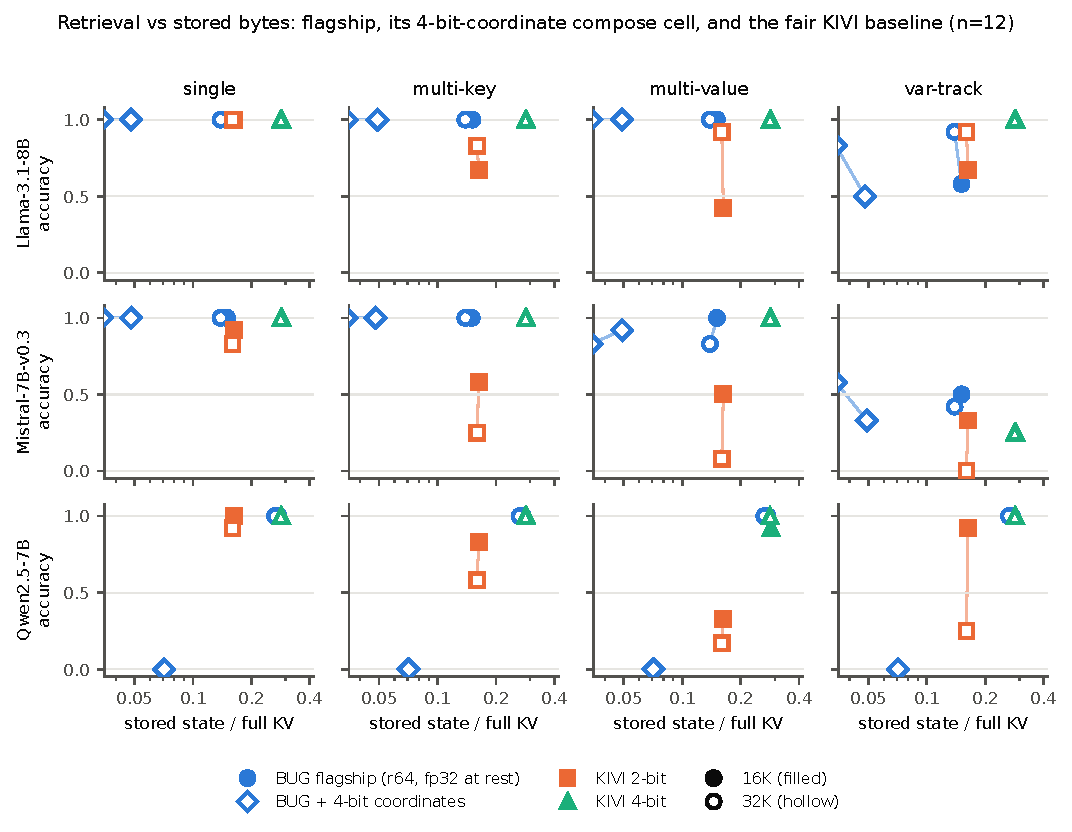
\includegraphics[width=\linewidth]{../figures/week19/fairquant.pdf}
\caption{Retrieval accuracy against honest stored bytes (log $x$), $n{=}12$ per
point, rows = families, columns = tasks. Filled markers are 16K, hollow 32K, joined
per arm. The flagship (blue circles, $0.15\times$ on Llama/Mistral, $0.27\times$ on
Qwen) sits beside the 2-bit KIVI arm (orange squares, $0.16\times$); the 4-bit arm
(aqua triangles, $0.28\times$) is perfect almost everywhere; the composed cell
(hollow blue diamonds, $0.048\times$) retrieves single/multi-key/multi-value on
Llama and Mistral below any 2-bit floor and collapses on Qwen. Source:
\texttt{scripts/w19\_figures.py} over the committed line-files.}
\label{fig:fairquant}
\end{figure}

\subsection{Moderate compression on realistic text}
\label{sec:realistic}
Two lines of evidence say the extreme-compression story is not a
synthetic-generator artifact. \textbf{(1) Realistic filler.} Re-running the
generator with WikiText filler instead of the fixed sentence pool, at 16K on Qwen
($n{=}12$), the flagship holds single-needle retrieval ($1.00$) while the
eviction baseline \texttt{ea-k0.1} ($0.100\times$) \emph{collapses to $0.00$ on
all four tasks}, and the low-rank baseline \texttt{palu-r0.5} loses
variable-tracking ($0.08$) and multi-value degrades ($0.83$); \texttt{think-c0.5}
holds single/multi-key but drops on multi-value/variable-tracking ($0.67$/$0.33$).
That the sub-$0.25\times$ eviction arm collapses on realistic text while the
flagship does not is the same ordering the synthetic generator shows, on
independent filler. \textbf{(2) LongBench.} On a LongBench~\citep{bai2024longbench}
document-QA probe (single Qasper document, $\sim$5.6K tokens), a
moderate-compression \texttt{bug-r128} scores F1 $0.221$ at $0.160\times$, ahead
of the sub-$0.25\times$ eviction arms (Expected~Attention-k0.25 $0.216$ at
$0.250\times$; -k0.1 $0.149$; SnapKV-k0.1 $0.136$) and of \texttt{palu-r0.25}
($0.073$); full KV is $0.259$. The LongBench point is one document (low power).
\textbf{(3) The official RULER anchor.} To confirm the numbers against a
generator we did not write, we ran the same arms on prompts produced by the
official NVIDIA RULER generator (commit \texttt{c3f5e3b}: its essay and noise
haystacks, needle types, templates, generation budgets and
\texttt{string\_match\_all} scoring; 12 records per task, Llama-3.1-8B, 16K;
Table~\ref{tab:official}). Three things transfer from our generator and one does
not. Eviction at $0.1\times$ collapses on every essay-haystack cell (mean $0.20$;
the flagship is paired-separated from it on 6 of 9 tasks, $p\le0.008$).
Single-needle retrieval is a tie between the flagship and the 2-bit quantizer.
The $0.29$--$0.75\times$ arms (4-bit KIVI, ThinK, Palu) are near-perfect. What
does \emph{not} transfer is the flagship's multi-value edge over 2-bit
quantization: on the official multi-value and multi-query prompts the paired
contrast is $1$ vs $1$ and $0$ vs $4$ discordant records, and over the nine tasks
the flagship averages $0.79$ against $0.87$ for the 2-bit arm at matched bytes
(no cell significant in either direction). The flagship's variable-tracking
weakness is confirmed and is where the larger arms separate from it ($0.33$ vs
$1.00$ for 4-bit KIVI, Palu and ThinK, $p=0.008$/$0.008$/$0.016$). Its $22$ misses (14 on the needle tasks at depths $0.15$--$0.95$, six of them at
depth $\le0.20$; and 8 variable-tracking chains) are front-loaded---six of
fourteen fall in the first ingest chunk---with a mid/late tail, misses the
near-lossless arms (4-bit KIVI, ThinK, Palu) do not make. We therefore state the matched-bytes
retrieval advantage of \S\ref{sec:quantbaseline} as a property of our generator
that the official suite does not reproduce at 16K, while the eviction collapse
and the single-needle parity do transfer.
% source: results/w19-a2-llama-lines.txt, results/w19_intervals/a2-llama-ruler-intervals.md, results/w19-a2-flagship-misses.md, docs/week19-official-ruler.md (a2-llama pod @c331ebd).

\begin{table}[htbp]
\centering
\caption{Official NVIDIA RULER (commit \texttt{c3f5e3b}) at 16K on Llama-3.1-8B,
12 records per task, accuracy under the official \texttt{string\_match\_all}
rule. s1--s3 = \texttt{niah\_single\_1/2/3} (noise, essay/numbers, essay/uuids);
mk1--3 = \texttt{niah\_multikey\_1/2/3}; mv/mq = multi-value/multi-query; vt =
variable tracking. Honest stored-bits ratios.}
\label{tab:official}
\small
\begin{tabular}{lcccccccccc|c}
\toprule
arm & stored & s1 & s2 & s3 & mk1 & mk2 & mk3 & mv & mq & vt & mean \\
\midrule
full KV & $1.00\times$ & 1.00 & 1.00 & 1.00 & 1.00 & 1.00 & 0.92 & 1.00 & 1.00 & 1.00 & 0.99 \\
\texttt{think-c0.5} & $0.75\times$ & 1.00 & 1.00 & 1.00 & 1.00 & 1.00 & 0.92 & 1.00 & 1.00 & 0.92 & 0.98 \\
\texttt{palu-r0.5} & $0.50\times$ & 1.00 & 1.00 & 1.00 & 1.00 & 1.00 & 0.92 & 0.42 & 0.92 & 1.00 & 0.92 \\
KIVI 4-bit & $0.29\times$ & 1.00 & 1.00 & 1.00 & 1.00 & 1.00 & 0.92 & 1.00 & 1.00 & 1.00 & 0.99 \\
KIVI 2-bit & $0.16\times$ & 1.00 & 1.00 & 0.83 & 1.00 & 0.92 & 0.58 & 0.83 & 1.00 & 0.67 & 0.87 \\
\texttt{bugSseed-r64-h256} & $0.15\times$ & 0.83 & 1.00 & 0.83 & 0.83 & 1.00 & 0.83 & 0.83 & 0.67 & 0.33 & 0.79 \\
\texttt{ea-k0.1} & $0.10\times$ & 1.00 & 0.17 & 0.00 & 0.33 & 0.00 & 0.00 & 0.00 & 0.00 & 0.33 & 0.20 \\
\bottomrule
\end{tabular}
\end{table}
% source: results/w18-g2-qwen-lines.txt (wikitext filler 16K Qwen: flagship single 1.00, ea-k0.1 0/0/0/0, palu-r0.5 1/1/0.83/0.08, think-c0.5 1/1/0.67/0.33); results/w11-goalA-lb-lines.txt (qasper).

\subsection{Composition with quantization (1B)}
\label{sec:frontier}
On Llama-3.2-1B (WikiText-2, ctx 1024), quantizing the gist coordinates to 4 bits
roughly halves stored state at negligible perplexity cost, and at a fixed budget
the composition beats pure low-rank (rank-64/4-bit $0.099\times$ vs rank-32/fp16
$0.097\times$ at lower perplexity): quantization and low-rank \emph{multiply}. But
under a \emph{fair} comparison---every mechanism quantized equally---BUG$\times$
TurboQuant is \textbf{competitive, not dominant}: Expected~Attention$\times$
TurboQuant and SnapKV$\times$TurboQuant sit on or ahead of BUG's Pareto frontier
through the mid-aggressive band ($0.08$--$0.18\times$), and pure 4-bit TurboQuant
is near-lossless at $0.25\times$. BUG is best only at the extreme edge
($<0.07\times$), where eviction becomes catastrophic and low-rank degrades
gracefully. (An earlier draft's ``beats SOTA at $10\times$'' compared quantized
BUG against fp16 eviction and is retracted.) This 1B study is why the honest
case rests on the extreme edge and the retrieval-per-byte niche, not on winning
mid-band perplexity---exactly the shape the 7B/8B fair quantization comparison
(\S\ref{sec:quantbaseline}) then confirms.
% source: docs/week4.md, main.tex(old) Week-4 fair-frontier paragraph, README Week-4.

\subsection{Memory: stored state vs.\ resident memory}
\label{sec:memory}
We bill memory two ways and report both.
\textbf{(1) Stored state} (float-equivalent, the numbers above): at $r{=}64$,
$0.085\times$ on Llama-8B and $0.149\times$ on Qwen-7B. Because the DLRA core
numerics are delicate (\S\ref{sec:siphon}), the gist is stored at fp32 at rest
while full KV is billed at fp16; the honest \emph{fp32-at-rest} ratios are
$\approx0.150\times$ (Llama-8B) and $\approx0.275\times$ (Qwen-7B). A
fp16-storable gist variant is not yet validated (\S\ref{sec:limits}).

\paragraph{The gist amortizes its overhead as $1/T$.} The flagship keeps the
whole coordinate buffer, so its stored state is a $\Theta(T)$ term (the $2r$
coordinates per token, slope $2r/n=0.125\times$ on $1024$-wide KV) \emph{plus} an
$O(rn+hn)$ overhead---$U$, the $h$-token exact tier, sinks and ring---that
\emph{amortizes} as $1/T$. So the honest ratio falls toward $2r/n$, not toward
zero: it drops from $0.149\times$ (16K) to $0.139\times$ (32K) on Qwen and
$0.085\times\!\to\!0.075\times$ (fp16-equiv) on Llama
(Tables~\ref{tab:xmodel},~\ref{tab:xmodel32}). We measured the next point
(Figure~\ref{fig:one_over_t}): at 64K on Llama the flagship's honest stored ratio
is $0.133\times$ ($0.151\to0.140\to0.133$ from 16K to 64K, fitting
$\mathrm{ratio}(T)\approx0.127+380/T$), $19\%$ under the 2-bit quantizer---whose
own ratio also amortizes a fixed residual ($0.163\to0.156\times$) rather than
staying exactly flat. At that point the flagship retrieves $1.00$ on all four
tasks ($n{=}8$; no contrast separates) where the 2-bit arm scores
$1.00/0.58/0.50/1.00$ and eviction at $0.1\times$ scores $1.00/0.67/0.83/1.00$
($n{=}12$; both also hold single/variable-tracking here), at perplexity $8.59$
against $8.15$ (2-bit and eviction), $7.27$ (4-bit) and $7.26$ (full KV, all to
scorer resolution). The distinctive property is therefore a lower \emph{asymptote}
($2r/n=0.125\times$ at fp32 coordinates vs the 2-bit arm's $0.156\times$, a $19\%$
margin, not an unbounded one) together with the retrieval difference at 64K; a
fp16-storable gist (\S\ref{sec:limits}) would put the asymptote at
$\approx0.063\times$, genuinely below the 2-bit floor. This $1/T$ term is also why
the persistence win (\S\ref{sec:memory} below) grows with context.
% source: results/w19-a4-llama-lines.txt (a4-llama pod @d15769d, A100-40GB: flagship n=8 1.00x4 @sbits 0.133 ppl 8.591; quant-2bit-kivi 1.00/0.58/0.50/1.00 @0.158 ppl 8.149; quant-4bit 1.00/0.83/1.00/0.58 @0.283 ppl 7.274; ea-k0.1 1.00/0.67/0.83/1.00 @0.100 ppl 8.149; full ppl 7.260).

\begin{figure}[htbp]
\centering
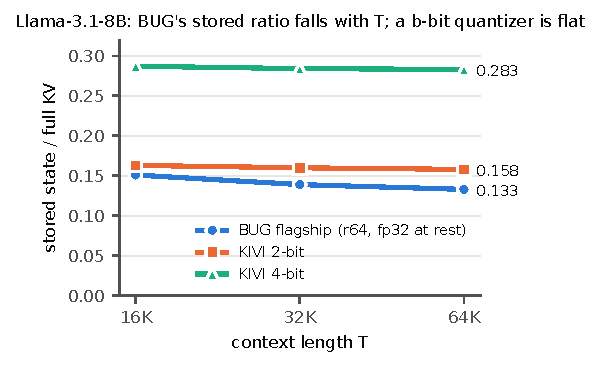
\includegraphics[width=0.6\linewidth]{../figures/week19/one_over_t.pdf}
\caption{Stored state as a fraction of full KV against context length on
Llama-3.1-8B (honest fp32-at-rest billing for BUG). The flagship's ratio falls with
$T$ as its $O(rn+hn)$ overhead amortizes, toward a $2r/n=0.125\times$ asymptote
(fit $0.127+380/T$); a $b$-bit quantizer is nearly flat at $b/16$ plus a small
amortizing residual.}
\label{fig:one_over_t}
\end{figure}
\textbf{(2) Resident memory} is \emph{not} the stored ratio. BUG is
reconstruct-then-attend: attention sees a full-length reconstruction, so the
decode-time reconstruction workspace is $\approx$ full KV---now measured on CUDA
(Llama-8B, \texttt{w16\_storage}): $0.982\times$ at 16K and $0.991\times$ at 32K
for \texttt{bugSseed-r64-h256} ($0.998$/$0.999\times$ for the pure gist
\texttt{bug-r64}), with the analytic--empirical footprint cross-check exact
(integrity $0$). This measured $\approx0.98\times$ workspace is exactly why a
naive peak-VRAM reading shows no win, and it implies analytically
(stored $+$ reconstruction workspace) a decode residency $\approx1.06\times$ full
KV---slightly worse than no compression; the full-KV arm's own decode peak was not
separately measured, so this is a sum, not a head-to-head.\footnote{The
released \texttt{w16\_storage} logs also carry a \texttt{peak\_ratio} of
$5$--$9\times$; this is peak process VRAM divided by the \emph{KV-cache} bytes, so
it is dominated by model weights (it halves as context doubles, $9.1\times$ at
16K vs $5.3\times$ at 32K) and is \emph{not} a residency-vs-full-KV metric. The
residency comparison is the workspace number ($\approx0.98\times$) plus stored
state.} Our only
end-to-end latency datum (1B, CPU) has \texttt{bug-r128} at $224.9$\,ms/token vs
full KV $204.5$\,ms/token ($\approx10\%$ slower). Realizing the stored-state
ratio as resident memory requires a fused factored attention kernel; we state
clearly that we have not built one, so on the resident axis eviction and ThinK
($0.75\times$ resident) currently beat BUG.

Where the stored-state ratio \emph{does} pay off today is persistence and
transfer, and this is now a \emph{measured} number rather than a projection.
On CUDA (Llama-8B, \texttt{w16\_storage}), the serialized cold-load size of
\texttt{bugSseed-r64-h256} is $0.150\times$ full KV at 16K and $0.139\times$ at
32K (pure gist \texttt{bug-r64}: $0.135\times$/$0.130\times$)---an $\approx
6.7$--$7.7\times$ smaller artifact to store, ship, or reload for prefix-cache
reuse and conversation resumption. Concretely, a serialized full KV at 32K
(Llama-8B, fp16) is $4.29$\,GB versus $\approx0.60$\,GB for \texttt{r64-h256};
the load-path win grows with context and with slower storage tiers. The
end-to-end cold start is now measured on the same card (Llama-8B, A100-40GB;
medians of five; persisted state = exactly the billed tensors, cores stored as
their diagonals): bringing a persisted cache back to attend-ready---warm page-cache read,
host-to-device copy, and BUG's reconstruction of the middle---takes
$\mathbf{0.13}$\,s at 16K ($325$\,MB) and $\mathbf{0.23}$\,s at 32K ($600$\,MB)
for \texttt{bugSseed-r64-h256}, against $1.23$\,s ($2.15$\,GB) and $2.35$\,s
($4.29$\,GB) for full KV: $\approx7\times$ fewer bytes and, on this pod, a
$9$--$10\times$ faster reload (the small artifact loads at a higher per-byte rate
than the multi-GB full cache). Two honest notes:
the reconstruction step is $0.04$--$0.08$\,s of that total (the rest is I/O), and
the 2-bit quantized cache of \S\ref{sec:quantbaseline} cold-starts in
$0.14$/$0.21$\,s at $336$/$671$\,MB---so the persistence win over full KV is
\emph{shared} with quantization at 16--32K. What separates them on this axis is
the $1/T$ term: BUG's persisted bytes fall from $0.151\times$ to $0.140\times$
between 16K and 32K while the quantizer holds $0.156\times$
(Figure~\ref{fig:coldstart}).

\begin{figure}[htbp]
\centering
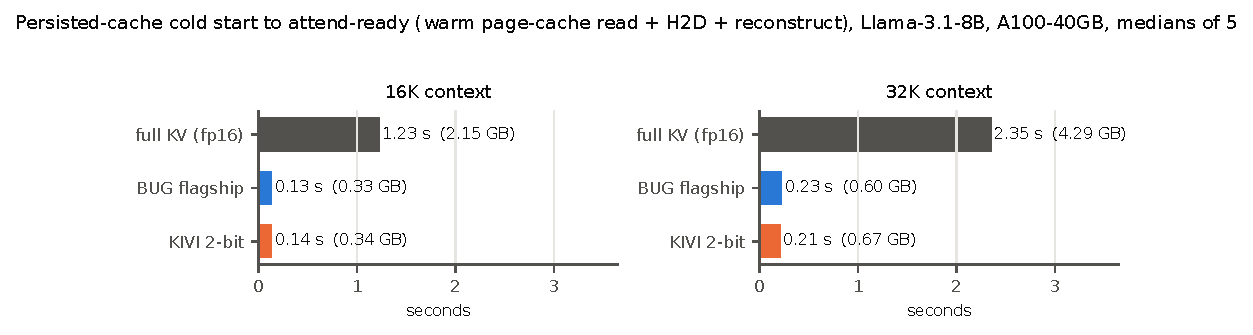
\includegraphics[width=\linewidth]{../figures/week19/coldstart.pdf}
\caption{Persisted-cache cold start to attend-ready on Llama-3.1-8B (A100-40GB,
medians of five): warm page-cache read + host-to-device + reconstruction. Bar labels give the
persisted size. Full KV takes $1.2$/$2.4$\,s at 16K/32K; the flagship and the 2-bit
quantized cache both take $0.1$--$0.2$\,s.}
\label{fig:coldstart}
\end{figure}
% source: results/w19-a3-llama2-lines.txt (w19_persist.py, SHA 5e8b275: 16K full 2147MB cold 1.226s | flagship 325MB 0.134s (load .067 h2d .028 ready .039) | kivi-2bit 336MB 0.137s; 32K full 4295MB 2.351s | flagship 600MB 0.227s | kivi-2bit 671MB 0.212s).
% source: results/w18-g5 (CUDA w16_storage: bugSseed-r64-h256 16K stored 0.084 coldload 0.150 workspace 0.982 peak 9.09; 32K stored 0.074 coldload 0.139 workspace 0.991; bug-r64 16K workspace 0.998 coldload 0.135; integrity 0). Latency/residency 1.06x from review-systems.md.

\FloatBarrier
\section{Limitations}
\label{sec:limits}
We lead with the two limitations that most constrain the claims.

\paragraph{Storage is not resident memory; no kernel yet.} As \S\ref{sec:memory}
states, the headline ratio is \emph{stored/persisted state}. Decode residency is
$\approx1.06\times$ full KV under reconstruct-then-attend, and the one latency
datum is $\approx10\%$ unfavorable. A fused low-rank attention kernel is the
missing piece that would turn stored state into resident savings; it is the
single most important systems item and is not built. The cache layout is also
single-sequence (batch size 1; \texttt{bug\_cache} assumes a $(1,H,T,D)$ shape),
so batched serving is out of scope for this paper.

\paragraph{Variable tracking on wide-KV models is unsolved.} On the two
$n{=}1024$ models, variable-tracking tops out at $0.58$ (Llama) / $0.50$
(Mistral) at 16K, while Qwen ($n{=}512$) reaches $1.00$ (Table~\ref{tab:xmodel}).
Following a \texttt{V0=\ldots; V1=V0; \ldots} chain needs several \emph{linked,
low-surprise} tokens retained together, but surprise selection provably keeps
\emph{sharp, isolated} needles---it protects the wrong tokens for chains. We
tested and \emph{refuted} the obvious fix (raising the exact-tier budget gives no
lift on real 7B/8B: Mistral $0.50\to0.25$, Llama $0.58\to0.58$), and two
memory-free alternatives failed a CPU probe. This is a real open problem---a
non-surprise retention mechanism for chains---not a solved axis.
% source: docs/week17-explained.md sec.2 (vt fix refuted), sec.1 (0.58/0.50/1.00).

\paragraph{Scale of the perplexity/composition study.} The full
fair-comparison frontier (\S\ref{sec:frontier}) and the near-oracle study are at
1B; at 7B/8B the fair comparison is the single-config flagship against the
2/4-bit quantizer (\S\ref{sec:quantbaseline}) and the one composed cell
(\S\ref{sec:subcliff}), not a swept frontier.

\paragraph{At matched bytes, 2-bit quantization is a strong competitor; 4-bit is
not separated.} The fair baseline (\S\ref{sec:quantbaseline}) ties the
flagship on single-needle retrieval everywhere, wins fluency on Mistral and Qwen,
and at 32K on Llama is not separated on any task. BUG's edge at $0.15\times$ is
confined to multi-value (all families) and, at 32K, multi-key on Mistral and
variable-tracking on Qwen. The 4-bit arm at about twice the bytes is not separated
from the flagship in any cell (the flagship leads its variable-tracking on Mistral
on point estimate, at half the bytes), and on Qwen---where the $n{=}512$ gist's
fp32-at-rest state costs $0.275\times$, the same bytes as 4-bit---the $r{=}64$
flagship is dominated outright. The band quantization cannot enter
(\S\ref{sec:subcliff}) holds on Llama and Mistral only, costs fluency, and fails
on Qwen. A fp16-storable gist (halving BUG's honest bytes) would change this
comparison materially and is the most valuable single follow-up.

\paragraph{Benchmark external validity: the official anchor cuts both ways.}
Most retrieval evidence uses an in-repo RULER-style generator. The official
RULER anchor (\S\ref{sec:realistic}, Llama 16K, 12 records per task) confirms
the eviction collapse and single-needle parity with 2-bit quantization, but it
does \emph{not} reproduce the multi-value edge over 2-bit quantization that our
generator shows, and on average the flagship trails the 2-bit arm there ($0.79$
vs $0.87$; no task separated). We therefore scope the matched-bytes retrieval
advantage to our generator's tasks and treat the official numbers as the
external-validity ceiling. The anchor covers one model and one context; a
three-family, 32K official grid and a flagship LongBench sweep remain open. The
composed sub-cliff cell (\S\ref{sec:subcliff}) has no official-anchor number at
all; its retrieval is our-generator-only.

\paragraph{Statistical firmness and provenance.} The 1B composition study is
lower-$n$, but the retrieval grids are now firm: the 16K and 32K cross-model
tables are $n{=}12$ and the marquee is $n{=}16$, from a September program run in
which pods were cloned by \emph{commit SHA} (not branch), stamped their git-SHA
and GPU/torch/CUDA environment into the harvested logs, and emitted per-trial hit
records (committed under \texttt{results/w18\_pertrial/} and
\texttt{results/w18\_harvest/}). The program spanned two commits---the
16K/32K flagship and quantization grids at \texttt{15678a7}, and the eviction,
filler, marquee-firming and storage grids at \texttt{b157acd}, differing only in
the quant-axis and plotting code, with the integrator/cache/RULER paths identical
and cross-pod-reproduced---rather than a single pod. The marquee retrieval and perplexity are same-pod
(\S\ref{sec:marquee}). The Week-19 additions (a quant-config diagnostic at \texttt{24ac22a}, the fair
quantization baseline at \texttt{6734afa}, sub-cliff composition at
\texttt{1cbc31f}, persistence at \texttt{5e8b275}, official anchor at
\texttt{c331ebd}, the 64K point at \texttt{d15769d}) follow the same SHA-pinned,
per-trial protocol, record their \texttt{optimum-quanto}/\texttt{hqq} versions in
\texttt{results/w19-env-provenance.txt}, and are paired with the Week-18 flagship
records needle-for-needle; the 64K flagship cells are $n{=}8$ (its comparators
$n{=}12$). The Week-19 GPU program was $\approx42$ A100-40GB pod-hours
($\approx\$39$); a full compute appendix and the 1B frontier's Week-15 provenance
(earlier material, not the September program) remain open.

\section{Conclusion}
\label{sec:conc}
We recast a numerical-analysis integrator---the rank-adaptive BUG scheme for
dynamical low-rank approximation---as an online, training-free, per-sequence KV
compressor: a near-oracle low-rank gist for fluency, a surprise-selected exact
tier for retrieval, and a warm-up seed for early context. Across three model
families it reaches perfect single/multi-value 16K retrieval with no detected
loss at $0.085$--$0.149\times$ float-equivalent stored state
($3.4$--$10\times$ under the channel-pruning/low-rank baselines
\texttt{think-c0.5}/\texttt{palu-r0.5}), and at 32K on the hardest task it beats
\texttt{think-c0.5} (Wilson-separated) and leads \texttt{palu-r0.5}
(not separated) at several-fold less stored state. As much as the frontier,
the contribution is the honest mechanistic map: the $r/n\approx0.25$ retrieval
wall, the rank-siphoning tier--gist interaction and its CKL-$\theta$-relative fix,
the wide-KV variable-tracking limitation, and the storage-vs-resident memory
distinction that scopes the systems claim. Against the fair 2-bit quantizer at matched bytes the method's edge narrows
to multi-value (and, at 32K, multi-key on Mistral and variable-tracking on Qwen)
retrieval, at a fluency cost, while 4-bit quantization at twice the bytes is not
separated from it; the one band no fixed-bit scalar quantizer can be configured to
enter is the composed gist-plus-4-bit-coordinates cell at $0.048\times$ on Llama
and Mistral (family-dependent, at a fluency cost). Low-rank tracking is an axis orthogonal to eviction and
quantization; a fp16-storable gist and a fused factored-attention kernel are the
program that would turn today's stored-state advantage into a deployed one.

\small
\bibliographystyle{plainnat}
\bibliography{refs}

\end{document}
